\documentclass[]{article}

\usepackage{graphicx,type1cm,eso-pic,color}
\usepackage[spanish]{babel} %%%% for


\makeatletter
          \AddToShipoutPicture{
            \setlength{\@tempdimb}{.95\paperwidth}
            \setlength{\@tempdimc}{.5\paperheight}
            \setlength{\unitlength}{1pt}
            \put(\strip@pt\@tempdimb,\strip@pt\@tempdimc){
        \makebox(0,0){\rotatebox{-90}{\textcolor[gray]{0.90}
        {\fontsize{.65cm}{.5cm}\selectfont{\rm Dae-Jin Lee}}}}
            }
        }
          \AddToShipoutPicture{
            \setlength{\@tempdimb}{.50\paperwidth}
            \setlength{\@tempdimc}{.95\paperheight}
            \setlength{\unitlength}{1pt}
            \put(\strip@pt\@tempdimb,\strip@pt\@tempdimc){
        \makebox(0,0){\rotatebox{0}{\textcolor[gray]{0.90}
        {\fontsize{.5cm}{.5cm}\selectfont{\rm Curso de Estad\'istica b\'asica para Data Scientist  - @datahack}}}}
            }
        }
\makeatother

\def\tightlist{}

\usepackage{lmodern}
\usepackage{amssymb,amsmath}
\usepackage{ifxetex,ifluatex}
\usepackage{fixltx2e} % provides \textsubscript
\ifnum 0\ifxetex 1\fi\ifluatex 1\fi=0 % if pdftex
  \usepackage[T1]{fontenc}
  \usepackage[utf8]{inputenc}
\else % if luatex or xelatex
  \ifxetex
    \usepackage{mathspec}
    \usepackage{xltxtra,xunicode}
  \else
    \usepackage{fontspec}
  \fi
  \defaultfontfeatures{Mapping=tex-text,Scale=MatchLowercase}
  \newcommand{\euro}{???}
\fi
% use upquote if available, for straight quotes in verbatim environments
\IfFileExists{upquote.sty}{\usepackage{upquote}}{}
% use microtype if available
\IfFileExists{microtype.sty}{%
\usepackage{microtype}
\UseMicrotypeSet[protrusion]{basicmath} % disable protrusion for tt fonts
}{}
\usepackage{color}
\usepackage{fancyvrb}
\newcommand{\VerbBar}{|}
\newcommand{\VERB}{\Verb[commandchars=\\\{\}]}
\DefineVerbatimEnvironment{Highlighting}{Verbatim}{commandchars=\\\{\}}
% Add ',fontsize=\small' for more characters per line
\usepackage{framed}
\definecolor{shadecolor}{RGB}{248,248,248}
\newenvironment{Shaded}{\begin{snugshade}}{\end{snugshade}}
\newcommand{\KeywordTok}[1]{\textcolor[rgb]{0.13,0.29,0.53}{\textbf{{#1}}}}
\newcommand{\DataTypeTok}[1]{\textcolor[rgb]{0.13,0.29,0.53}{{#1}}}
\newcommand{\DecValTok}[1]{\textcolor[rgb]{0.00,0.00,0.81}{{#1}}}
\newcommand{\BaseNTok}[1]{\textcolor[rgb]{0.00,0.00,0.81}{{#1}}}
\newcommand{\FloatTok}[1]{\textcolor[rgb]{0.00,0.00,0.81}{{#1}}}
\newcommand{\ConstantTok}[1]{\textcolor[rgb]{0.00,0.00,0.00}{{#1}}}
\newcommand{\CharTok}[1]{\textcolor[rgb]{0.31,0.60,0.02}{{#1}}}
\newcommand{\SpecialCharTok}[1]{\textcolor[rgb]{0.00,0.00,0.00}{{#1}}}
\newcommand{\StringTok}[1]{\textcolor[rgb]{0.31,0.60,0.02}{{#1}}}
\newcommand{\VerbatimStringTok}[1]{\textcolor[rgb]{0.31,0.60,0.02}{{#1}}}
\newcommand{\SpecialStringTok}[1]{\textcolor[rgb]{0.31,0.60,0.02}{{#1}}}
\newcommand{\ImportTok}[1]{{#1}}
\newcommand{\CommentTok}[1]{\textcolor[rgb]{0.56,0.35,0.01}{\textit{{#1}}}}
\newcommand{\DocumentationTok}[1]{\textcolor[rgb]{0.56,0.35,0.01}{\textbf{\textit{{#1}}}}}
\newcommand{\AnnotationTok}[1]{\textcolor[rgb]{0.56,0.35,0.01}{\textbf{\textit{{#1}}}}}
\newcommand{\CommentVarTok}[1]{\textcolor[rgb]{0.56,0.35,0.01}{\textbf{\textit{{#1}}}}}
\newcommand{\OtherTok}[1]{\textcolor[rgb]{0.56,0.35,0.01}{{#1}}}
\newcommand{\FunctionTok}[1]{\textcolor[rgb]{0.00,0.00,0.00}{{#1}}}
\newcommand{\VariableTok}[1]{\textcolor[rgb]{0.00,0.00,0.00}{{#1}}}
\newcommand{\ControlFlowTok}[1]{\textcolor[rgb]{0.13,0.29,0.53}{\textbf{{#1}}}}
\newcommand{\OperatorTok}[1]{\textcolor[rgb]{0.81,0.36,0.00}{\textbf{{#1}}}}
\newcommand{\BuiltInTok}[1]{{#1}}
\newcommand{\ExtensionTok}[1]{{#1}}
\newcommand{\PreprocessorTok}[1]{\textcolor[rgb]{0.56,0.35,0.01}{\textit{{#1}}}}
\newcommand{\AttributeTok}[1]{\textcolor[rgb]{0.77,0.63,0.00}{{#1}}}
\newcommand{\RegionMarkerTok}[1]{{#1}}
\newcommand{\InformationTok}[1]{\textcolor[rgb]{0.56,0.35,0.01}{\textbf{\textit{{#1}}}}}
\newcommand{\WarningTok}[1]{\textcolor[rgb]{0.56,0.35,0.01}{\textbf{\textit{{#1}}}}}
\newcommand{\AlertTok}[1]{\textcolor[rgb]{0.94,0.16,0.16}{{#1}}}
\newcommand{\ErrorTok}[1]{\textcolor[rgb]{0.64,0.00,0.00}{\textbf{{#1}}}}
\newcommand{\NormalTok}[1]{{#1}}
\usepackage{graphicx}
\makeatletter
\def\maxwidth{\ifdim\Gin@nat@width>\linewidth\linewidth\else\Gin@nat@width\fi}
\def\maxheight{\ifdim\Gin@nat@height>\textheight\textheight\else\Gin@nat@height\fi}
\makeatother
% Scale images if necessary, so that they will not overflow the page
% margins by default, and it is still possible to overwrite the defaults
% using explicit options in \includegraphics[width, height, ...]{}
\setkeys{Gin}{width=\maxwidth,height=\maxheight,keepaspectratio}
\ifxetex
  \usepackage[setpagesize=false, % page size defined by xetex
              unicode=false, % unicode breaks when used with xetex
              xetex]{hyperref}
\else
  \usepackage[unicode=true]{hyperref}
\fi
\hypersetup{breaklinks=true,
            bookmarks=true,
            pdfauthor={Dae-Jin Lee \textless{} lee.daejin@gmail.com \textgreater{}},
            pdftitle={Curso de Estadística básica para Data Scientists},
            colorlinks=true,
            citecolor=blue,
            urlcolor=blue,
            linkcolor=magenta,
            pdfborder={0 0 0}}
\urlstyle{same}  % don't use monospace font for urls
\setlength{\parindent}{0pt}
\setlength{\parskip}{6pt plus 2pt minus 1pt}
\setlength{\emergencystretch}{3em}  % prevent overfull lines
\setcounter{secnumdepth}{5}

\title{\textbf{Curso de Estadística básica para Data Scientists}}
\author{Dae-Jin Lee \textless{}
\href{mailto:lee.daejin@gmail.com}{\nolinkurl{lee.daejin@gmail.com}}
\textgreater{}}
\date{TEMA 7. Regresión para datos binarios y de conteo}

\usepackage{amsfonts}
\usepackage{amsmath}
\usepackage{amssymb}
\usepackage{natbib}
%\usepackage[T1]{fontenc}
\usepackage{latexsym}
\usepackage{graphicx}
\usepackage{caption}
\usepackage{subcaption}
\usepackage{color}
\usepackage{algorithm2e}
%%
%     Definitions
%
\newcommand{\tri}{\bigtriangleup}
\newcommand{\Xp}{X^\prime}
\newcommand{\E}{\mbox{E}}
\newcommand{\Hh}{\mbox{H}}
\newcommand{\V}{\mbox{Var}}
\newcommand{\tr}{\mbox{tr}}
\newcommand{\CV}{\mbox{CV}}
\newcommand{\GCV}{\mbox{GCV}}
\newcommand{\AIC}{\mbox{AIC}}
\newcommand{\ph}{\phantom{0}}
\newcommand{\half}{\mbox{${1\over2}$}}
\newcommand{\bfzero}{\boldsymbol{0}}
\newcommand{\bfone}{\boldsymbol{1}}

\newcommand{\bfa}{\boldsymbol{a}}
\newcommand{\bfb}{\boldsymbol{b}}
\newcommand{\bfe}{\boldsymbol{e}}
\newcommand{\bff}{\boldsymbol{f}}
\newcommand{\bfg}{\boldsymbol{g}}
\newcommand{\bfs}{\boldsymbol{s}}
\newcommand{\bfu}{\boldsymbol{u}}
\newcommand{\bfx}{\boldsymbol{x}}
\newcommand{\bfy}{\boldsymbol{y}}
\newcommand{\bfz}{\boldsymbol{z}}

\newcommand{\bfA}{\boldsymbol{A}}
\newcommand{\bfB}{\boldsymbol{B}}
\newcommand{\bfC}{\boldsymbol{C}}
\newcommand{\bfD}{\boldsymbol{D}}
\newcommand{\bfF}{\boldsymbol{F}}
\newcommand{\bfG}{\boldsymbol{G}}
\newcommand{\bfH}{\boldsymbol{H}}
\newcommand{\bfI}{\boldsymbol{I}}
\newcommand{\bfM}{\boldsymbol{M}}
\newcommand{\bfP}{\boldsymbol{P}}
\newcommand{\bfQ}{\boldsymbol{Q}}
\newcommand{\bfR}{\boldsymbol{R}}
\newcommand{\bfS}{\boldsymbol{S}}
\newcommand{\bfT}{\boldsymbol{T}}
\newcommand{\bfU}{\boldsymbol{U}}
\newcommand{\bfV}{\boldsymbol{V}}
\newcommand{\bfW}{\boldsymbol{W}}
\newcommand{\bfX}{\boldsymbol{X}}
\newcommand{\bfY}{\boldsymbol{Y}}
\newcommand{\bfZ}{\boldsymbol{Z}}


\newcommand{\bfalpha}{\boldsymbol{\alpha}}
\newcommand{\bfbeta}{\boldsymbol{\beta}}
\newcommand{\bfepsilon}{\boldsymbol{\epsilon}}
\newcommand{\bfgamma}{\boldsymbol{\gamma}}
\newcommand{\bfGamma}{\boldsymbol{\Gamma}}
\newcommand{\bfmu}{\boldsymbol{\mu}}
\newcommand{\bfeta}{\boldsymbol{\eta}}
\newcommand{\bfrho}{\boldsymbol{\rho}}
\newcommand{\bftheta}{\boldsymbol{\theta}}
\newcommand{\bfxi}{\boldsymbol{\xi}}
\newcommand{\bftau}{\boldsymbol{\tau}}
\newcommand{\bflambda}{\boldsymbol{\lambda}}
\newcommand{\bfsigma}{\boldsymbol{\sigma}}
\newcommand{\bfLambda}{\boldsymbol{\Lambda}}
\newcommand{\bfSigma}{\boldsymbol{\Sigma}}

\renewcommand{\theequation}{\thesection.\arabic{equation}}
\numberwithin{equation}{section}

\begin{document}
\maketitle

{
\hypersetup{linkcolor=black}
\setcounter{tocdepth}{2}
\tableofcontents
}
\newpage

\href{https://idaejin.github.io/bcam-courses/R/datahack/}{Regresar a la
página principal}

\section{Logistic regression}\label{logistic-regression}

A logistic regression is typically used when there is one dichotomous
outcome variable (such as winning or losing), and a continuous predictor
variable which is related to the probability or odds of the outcome
variable. It can also be used with categorical predictors, and with
multiple predictors.

\subsection{ESR and Plasma Proteins}\label{esr-and-plasma-proteins}

The erythrocyte sedimentation rate (ESR) is the rate at which red blood
cells (erythrocytes) settle out of suspension in blood plasma, when
measured under standard conditions. If the ESR increases when the level
of certain proteins in the blood plasma rise in association with
conditions such as rheumatic diseases, chronic infections and malignant
diseases, its determination might be useful in screening blood samples
taken from people suspected of suffering from one of the conditions
mentioned. The absolute value of the ESR is not of great importance;
rather, less than 20mm/hr indicates a ``healthy'' individual. To assess
whether the ESR is a useful diagnostic tool, the question of interest is
whether there is any association between the probability of an ESR
reading greater than 20mm/hr and the levels of the two plasma proteins.
If there is not then the determination of ESR would not be useful for
diagnostic purposes. A data frame with 32 observations on the following
3 variables.

\begin{itemize}
\tightlist
\item
  \texttt{fibrinogen} the fibrinogen level in the blood.
\item
  \texttt{globulin} the globulin level in the blood.
\item
  \texttt{ESR} the erythrocyte sedimentation rate, either less or
  greater 20 mm / hour.
\end{itemize}

\begin{Shaded}
\begin{Highlighting}[]
\KeywordTok{data}\NormalTok{(}\StringTok{"plasma"}\NormalTok{, }\DataTypeTok{package =} \StringTok{"HSAUR"}\NormalTok{)}
\KeywordTok{head}\NormalTok{(plasma)}
\end{Highlighting}
\end{Shaded}

\begin{verbatim}
##   fibrinogen globulin      ESR
## 1       2.52       38 ESR < 20
## 2       2.56       31 ESR < 20
## 3       2.19       33 ESR < 20
## 4       2.18       31 ESR < 20
## 5       3.41       37 ESR < 20
## 6       2.46       36 ESR < 20
\end{verbatim}

\begin{Shaded}
\begin{Highlighting}[]
\KeywordTok{layout}\NormalTok{(}\KeywordTok{matrix}\NormalTok{(}\DecValTok{1}\NormalTok{:}\DecValTok{2}\NormalTok{, }\DataTypeTok{ncol =} \DecValTok{2}\NormalTok{))}
\KeywordTok{boxplot}\NormalTok{(fibrinogen ~}\StringTok{ }\NormalTok{ESR, }\DataTypeTok{data =} \NormalTok{plasma, }\DataTypeTok{varwidth =} \OtherTok{TRUE}\NormalTok{, }\DataTypeTok{main=}\StringTok{"Fibrinogen level in the blood"}\NormalTok{)}
\KeywordTok{boxplot}\NormalTok{(globulin ~}\StringTok{ }\NormalTok{ESR, }\DataTypeTok{data =} \NormalTok{plasma, }\DataTypeTok{varwidth =} \OtherTok{TRUE}\NormalTok{, }\DataTypeTok{main=}\StringTok{"Globulin level in the blood"}\NormalTok{)}
\end{Highlighting}
\end{Shaded}

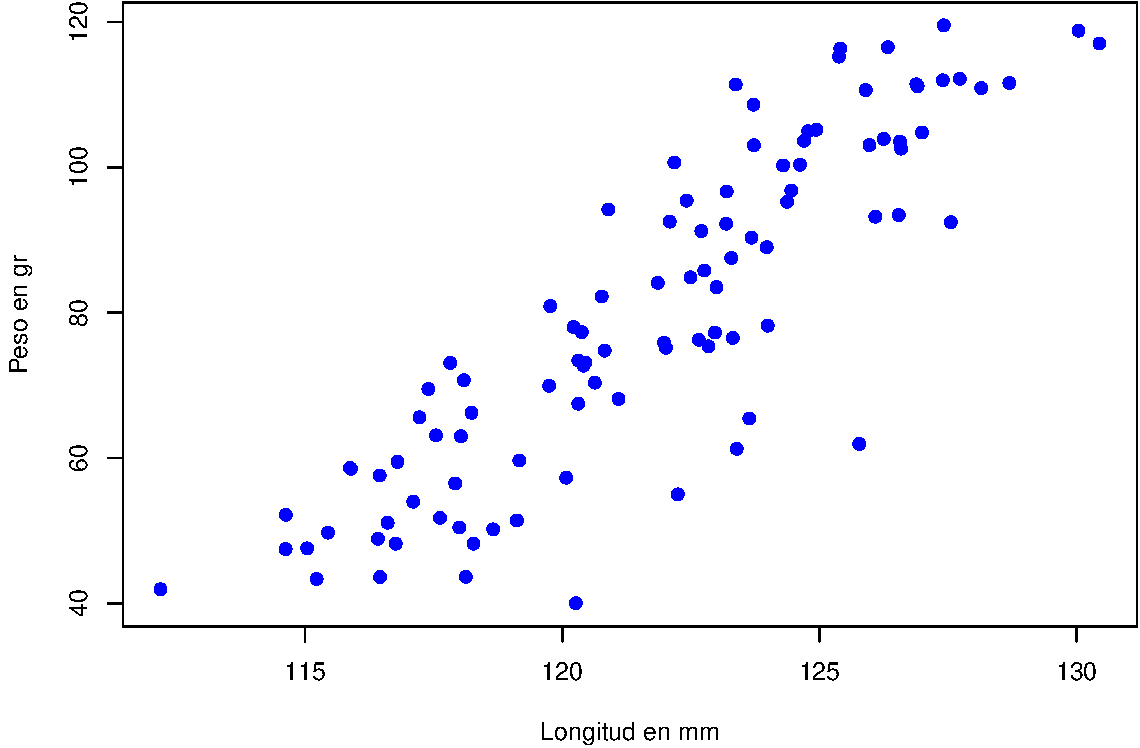
\includegraphics{tema7_files/figure-latex/unnamed-chunk-2-1.pdf}

The question of interest is whether there is any association between the
probability of an ESR reading greater than 20mm/hr and the levels of the
two plasma proteins. If there is not then the determination of ESR would
not be useful for diagnostic purposes.

Since the response variable is binary, a multiple regression model is
not suitable for a regression analysis.

We may write \[
\mathbb{P}\mbox{r}(y_i=1)=\pi_i \qquad \mathbb{P}\mbox{r}(y_i=0)=1-\pi_i
\]

Normally, we will have a set of covariates \(X=(x_1,..., x_p)\)
associated with each individual, and our goal will be to investigate the
relationship between the response probability \(\pi=\pi(X)\) and the
explanatory variables.

So instead of modelling the expected value of the response directly as a
linear function of explanatory variables, a suitable transformation is
modelled. In this case the most suitable transformation is the logistic
or logit function of \(\pi\) leading to the model

\[
  \mbox{logit}(\pi) = \mbox{logit}\left(\frac{\pi}{1-\pi}\right) = \beta_0 + \beta_1x_1 + ... + \beta_p x_p
\]

The logit of a probability is simply the log of the odds of the response
taking the value one or logit transformation, of p:
\(logit(p) = \log(p/1-p)\). Logit is sometimes called ``log odds.''
Because of the properties of odds given in the list above, the logit has
these properties:

\begin{itemize}
\tightlist
\item
  If \texttt{odds(y=1s)\ =\ 1}, then \texttt{logit(p)\ =\ 0}.
\item
  If \texttt{odds(y=1)\ \textless{}\ 1}, then
  \texttt{logit(p)\ \textless{}\ 0}.
\item
  If \texttt{odds(y=1)\ \textgreater{}\ 1}, then
  \texttt{logit(p)\ \textgreater{}\ 0}.
\end{itemize}

The logit transform fails if p = 0`.

When the response is a binary (dichotomous) variable, and x is numeric,
logistic regression fits a logistic curve to the relationship between
\(x\) and \(y\). Hence, logistic regression is linear regression on the
logit transform of y, where y is the proportion (or probability) of
success at each value of x. However, you should avoid the temptation to
do a traditional least-squares regression at this point, as neither the
normality nor the homoscedasticity assumption will be met.

\begin{Shaded}
\begin{Highlighting}[]
\NormalTok{x <-}\StringTok{ }\KeywordTok{seq}\NormalTok{(-}\DecValTok{6}\NormalTok{,}\DecValTok{6}\NormalTok{,}\FloatTok{0.01}\NormalTok{)}
\NormalTok{logistic <-}\StringTok{ }\KeywordTok{exp}\NormalTok{(x)/(}\DecValTok{1}\NormalTok{+}\KeywordTok{exp}\NormalTok{(x))}
\KeywordTok{plot}\NormalTok{(x,logistic,}\DataTypeTok{t=}\StringTok{'l'}\NormalTok{,}\DataTypeTok{main=}\StringTok{"Logistic curve"}\NormalTok{,}\DataTypeTok{ylab=}\StringTok{""}\NormalTok{)}
\KeywordTok{abline}\NormalTok{(}\DataTypeTok{h=}\KeywordTok{c}\NormalTok{(}\DecValTok{0}\NormalTok{,}\FloatTok{0.5}\NormalTok{,}\DecValTok{1}\NormalTok{),}\DataTypeTok{v=}\DecValTok{0}\NormalTok{,}\DataTypeTok{col=}\StringTok{"grey"}\NormalTok{)}
\KeywordTok{points}\NormalTok{(}\DecValTok{0}\NormalTok{,}\FloatTok{0.5}\NormalTok{,}\DataTypeTok{pch=}\DecValTok{19}\NormalTok{,}\DataTypeTok{col=}\DecValTok{2}\NormalTok{)}
\end{Highlighting}
\end{Shaded}

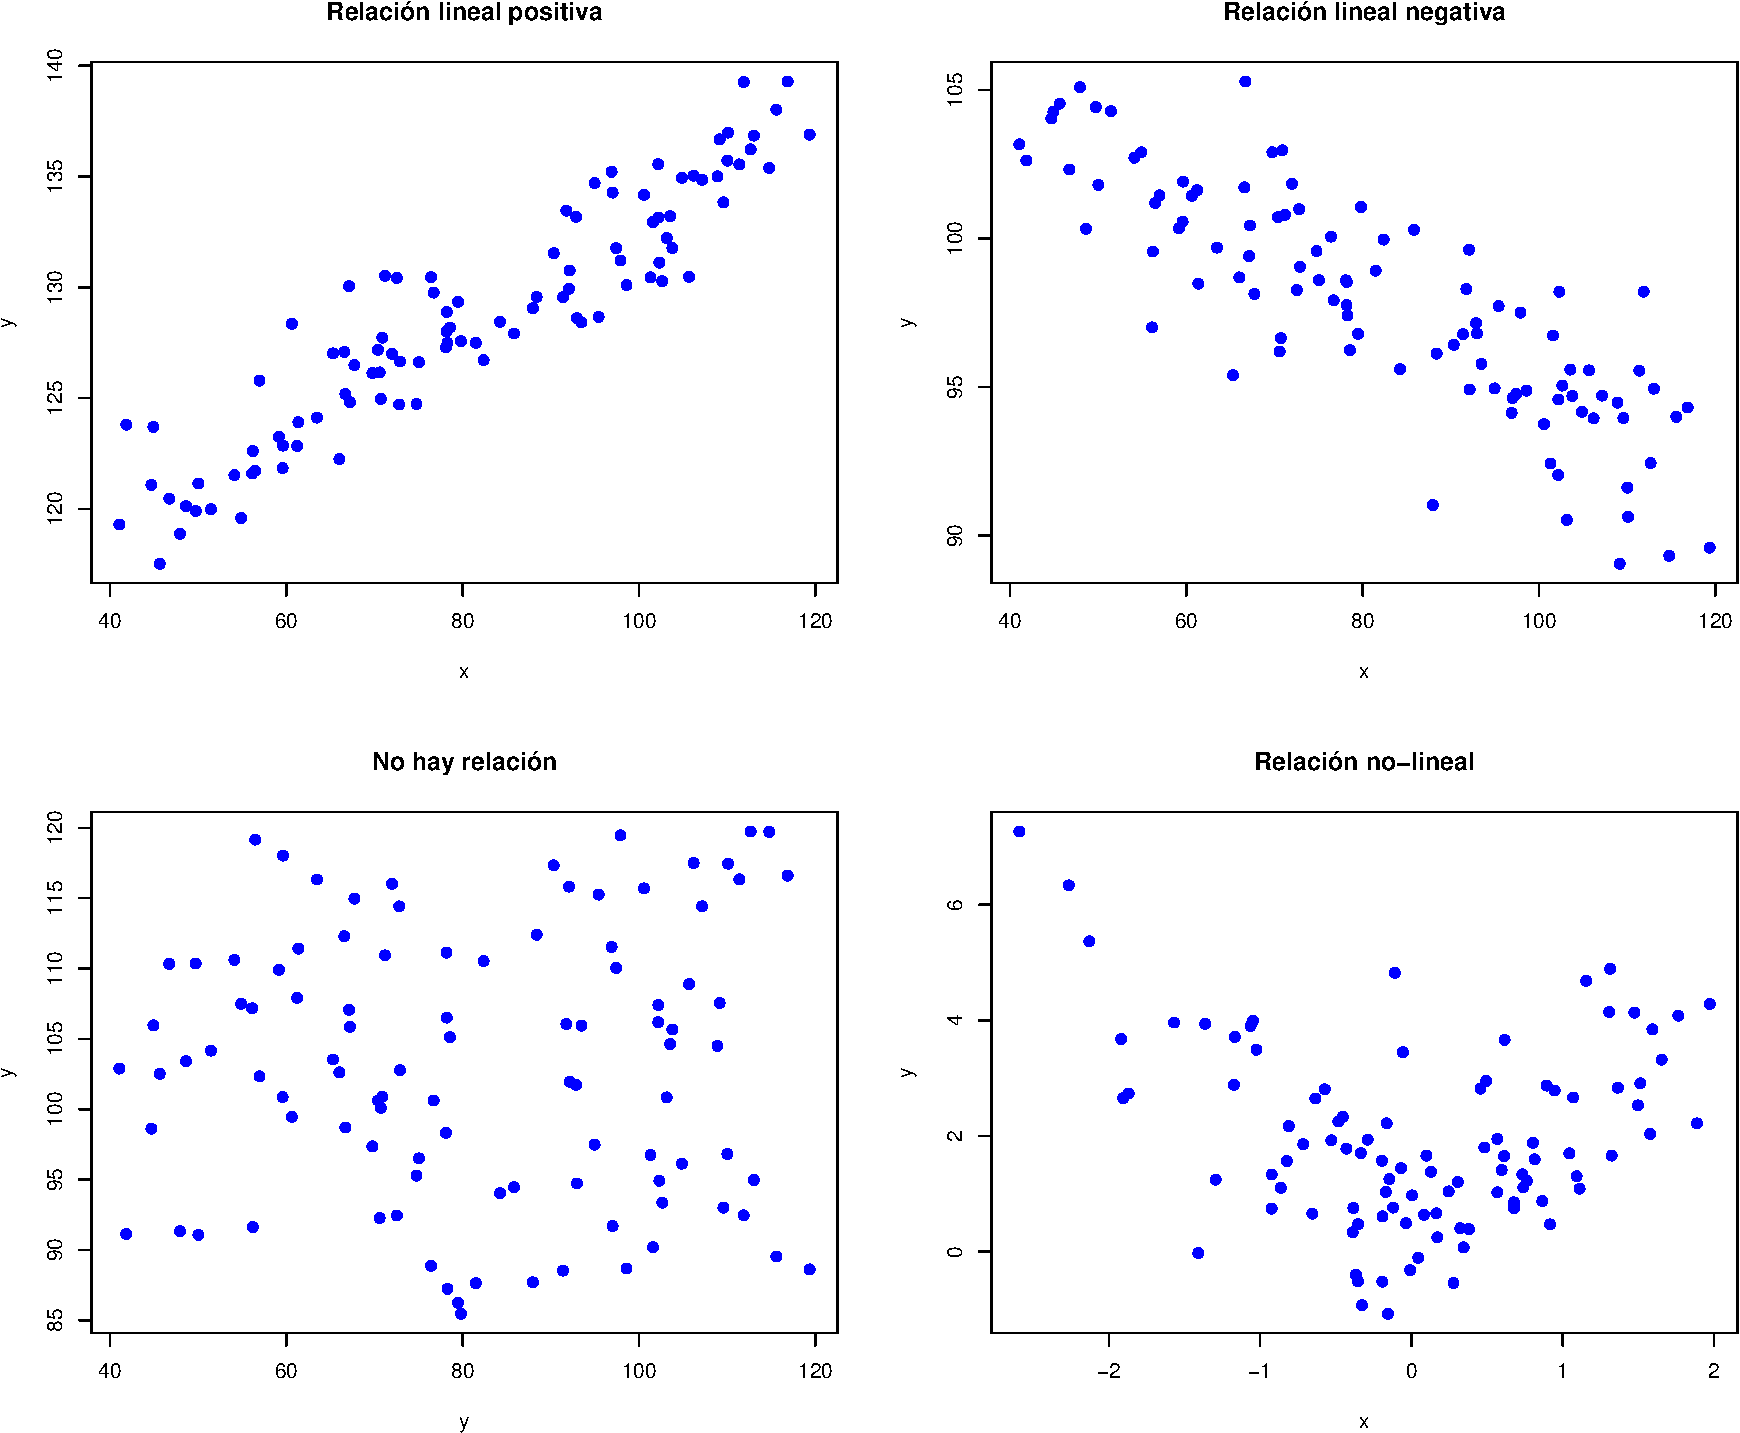
\includegraphics{tema7_files/figure-latex/unnamed-chunk-3-1.pdf}

Logistic regression model in \texttt{R} can be fitted using the function
\texttt{glm}. First, we start with a model that includes only a single
predictor \texttt{fibrinogen}

\begin{Shaded}
\begin{Highlighting}[]
\NormalTok{plasma_glm_1 <-}\StringTok{ }\KeywordTok{glm}\NormalTok{(ESR ~}\StringTok{ }\NormalTok{fibrinogen, }\DataTypeTok{data =} \NormalTok{plasma,}\DataTypeTok{family =} \KeywordTok{binomial}\NormalTok{())}
\KeywordTok{summary}\NormalTok{(plasma_glm_1)}
\end{Highlighting}
\end{Shaded}

\begin{verbatim}
## 
## Call:
## glm(formula = ESR ~ fibrinogen, family = binomial(), data = plasma)
## 
## Deviance Residuals: 
##     Min       1Q   Median       3Q      Max  
## -0.9298  -0.5399  -0.4382  -0.3356   2.4794  
## 
## Coefficients:
##             Estimate Std. Error z value Pr(>|z|)  
## (Intercept)  -6.8451     2.7703  -2.471   0.0135 *
## fibrinogen    1.8271     0.9009   2.028   0.0425 *
## ---
## Signif. codes:  0 '***' 0.001 '**' 0.01 '*' 0.05 '.' 0.1 ' ' 1
## 
## (Dispersion parameter for binomial family taken to be 1)
## 
##     Null deviance: 30.885  on 31  degrees of freedom
## Residual deviance: 24.840  on 30  degrees of freedom
## AIC: 28.84
## 
## Number of Fisher Scoring iterations: 5
\end{verbatim}

We see that the regression coefficient for \texttt{fibrinogen} is
significant at the \(5\%\) level. An increase of one unit in this
variable increases the log-odds in favour of an ESR value greater than
20 by an estimated \(1.83\) with \(95\%\) confidence interval.

\begin{Shaded}
\begin{Highlighting}[]
\KeywordTok{confint}\NormalTok{(plasma_glm_1,}\DataTypeTok{parm=}\StringTok{"fibrinogen"}\NormalTok{)}
\end{Highlighting}
\end{Shaded}

\begin{verbatim}
## Waiting for profiling to be done...
\end{verbatim}

\begin{verbatim}
##     2.5 %    97.5 % 
## 0.3387619 3.9984921
\end{verbatim}

These values are more helpful if converted to the corresponding values
for the odds themselves by exponentiating the estimate

\begin{Shaded}
\begin{Highlighting}[]
\KeywordTok{exp}\NormalTok{(}\KeywordTok{coef}\NormalTok{(plasma_glm_1)[}\StringTok{"fibrinogen"}\NormalTok{])}
\end{Highlighting}
\end{Shaded}

\begin{verbatim}
## fibrinogen 
##   6.215715
\end{verbatim}

and the confidence interval

\begin{Shaded}
\begin{Highlighting}[]
\KeywordTok{exp}\NormalTok{(}\KeywordTok{confint}\NormalTok{(plasma_glm_1, }\DataTypeTok{parm =} \StringTok{"fibrinogen"}\NormalTok{))}
\end{Highlighting}
\end{Shaded}

\begin{verbatim}
## Waiting for profiling to be done...
\end{verbatim}

\begin{verbatim}
##     2.5 %    97.5 % 
##  1.403209 54.515884
\end{verbatim}

The confidence interval is very wide because there are few observations
overall and very few where the ESR value is greater than 20.
Nevertheless it seems likely that increased values of fibrinogen lead to
a greater probability of an ESR value greater than 20. We can now fit a
logistic regression model that includes both explanatory variables using
the code

\begin{Shaded}
\begin{Highlighting}[]
\NormalTok{plasma_glm_2 <-}\StringTok{ }\KeywordTok{glm}\NormalTok{(ESR ~}\StringTok{ }\NormalTok{fibrinogen +}\StringTok{ }\NormalTok{globulin, }\DataTypeTok{data =} \NormalTok{plasma,}\DataTypeTok{family =} \KeywordTok{binomial}\NormalTok{())}
\KeywordTok{summary}\NormalTok{(plasma_glm_2)}
\end{Highlighting}
\end{Shaded}

\begin{verbatim}
## 
## Call:
## glm(formula = ESR ~ fibrinogen + globulin, family = binomial(), 
##     data = plasma)
## 
## Deviance Residuals: 
##     Min       1Q   Median       3Q      Max  
## -0.9683  -0.6122  -0.3458  -0.2116   2.2636  
## 
## Coefficients:
##             Estimate Std. Error z value Pr(>|z|)  
## (Intercept) -12.7921     5.7963  -2.207   0.0273 *
## fibrinogen    1.9104     0.9710   1.967   0.0491 *
## globulin      0.1558     0.1195   1.303   0.1925  
## ---
## Signif. codes:  0 '***' 0.001 '**' 0.01 '*' 0.05 '.' 0.1 ' ' 1
## 
## (Dispersion parameter for binomial family taken to be 1)
## 
##     Null deviance: 30.885  on 31  degrees of freedom
## Residual deviance: 22.971  on 29  degrees of freedom
## AIC: 28.971
## 
## Number of Fisher Scoring iterations: 5
\end{verbatim}

The coefficient for gamma globulin is not significantly different from
zero.

Both nested models can be compared using a likelihood ratio test with
\texttt{anova} function

\begin{Shaded}
\begin{Highlighting}[]
\KeywordTok{anova}\NormalTok{(plasma_glm_1, plasma_glm_2, }\DataTypeTok{test =} \StringTok{"Chisq"}\NormalTok{)}
\end{Highlighting}
\end{Shaded}

\begin{verbatim}
## Analysis of Deviance Table
## 
## Model 1: ESR ~ fibrinogen
## Model 2: ESR ~ fibrinogen + globulin
##   Resid. Df Resid. Dev Df Deviance Pr(>Chi)
## 1        30     24.840                     
## 2        29     22.971  1   1.8692   0.1716
\end{verbatim}

So we conclude that gamma globulin is not associated with ESR level.

The plot clearly shows the increasing probability of an ESR value above
20 (larger circles) as the values of fibrinogen, and to a lesser extent,
gamma globulin, increase.

\begin{Shaded}
\begin{Highlighting}[]
\NormalTok{prob <-}\StringTok{ }\KeywordTok{predict}\NormalTok{(plasma_glm_2,}\DataTypeTok{type=}\StringTok{"response"}\NormalTok{)}
\KeywordTok{plot}\NormalTok{(globulin ~}\StringTok{ }\NormalTok{fibrinogen, }\DataTypeTok{data =} \NormalTok{plasma, }\DataTypeTok{xlim =} \KeywordTok{c}\NormalTok{(}\DecValTok{2}\NormalTok{, }\DecValTok{6}\NormalTok{),}\DataTypeTok{ylim =} \KeywordTok{c}\NormalTok{(}\DecValTok{25}\NormalTok{, }\DecValTok{55}\NormalTok{), }\DataTypeTok{pch =} \StringTok{"."}\NormalTok{)}
\KeywordTok{symbols}\NormalTok{(plasma$fibrinogen, plasma$globulin, }\DataTypeTok{circles =} \NormalTok{prob,}\DataTypeTok{add =} \OtherTok{TRUE}\NormalTok{)}
\end{Highlighting}
\end{Shaded}

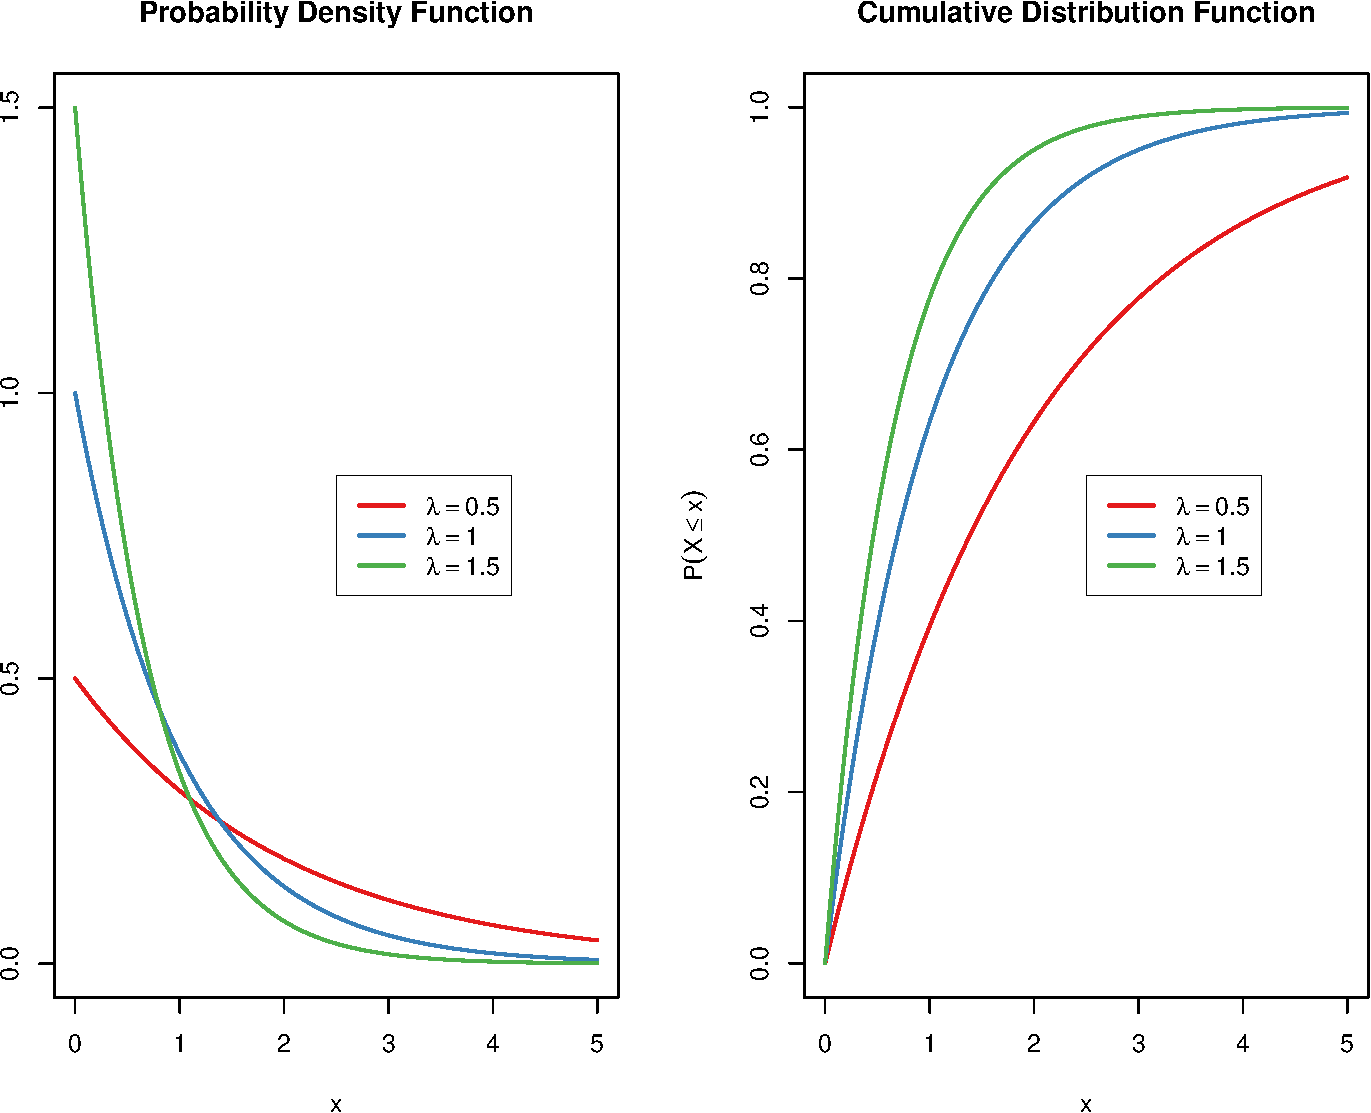
\includegraphics{tema7_files/figure-latex/unnamed-chunk-10-1.pdf}

\end{document}